\documentclass{article}

% Language setting
% Replace `english' with e.g. `spanish' to change the document language
\usepackage[french]{babel}
\usepackage[T1]{fontenc} 

% Set page size and margins
% Replace `letterpaper' with `a4paper' for UK/EU standard size
\usepackage[a4paper,top=2cm,bottom=2cm,left=2cm,right=2cm,marginparwidth=1.75cm]{geometry}
\setlength{\parindent}{0em}
\setlength{\parskip}{0.8em}
% \usepackage[skip=10pt plus1pt, indent=0pt]{parskip}

% Useful packages
\usepackage{float}
\usepackage{amsmath}
\usepackage{graphicx}
\graphicspath{{./images/}} %Setting the graphicspath
\usepackage[colorlinks=true, allcolors=blue]{hyperref}

\usepackage{tikz}

% To create code block
\usepackage{framed,verbatim}
\definecolor{shadecolor}{gray}{0.9}
\newenvironment{code}%
   {\snugshade\verbatim}%
   {\endverbatim\endsnugshade}
%

%%%%%%%%%% Début du doc %%%%%%%%%%

\title{Analyse de malware}
\author{Bastien Pesme,  Youssef Ifri}

\begin{document}
\maketitle

% \begin{abstract}
% Your abstract.
% \end{abstract}

\section{A Faire}
rendre sur un git public
- dossier de notre malware
- slides de l'analyse
- petit résumé de notre malware (notre code) : comment on a fait, comment on a caché,... (une page environ)
- comment lancer le malware
- donner la vraie clé

dans les slides : donner ce qu'on a vu du code
antidebug
chiffrement
automodification
outils utilisés
etc...

\section*{Introduction}

\section{Analyse Statique}

\subsection{analyse antivirus}
\subsection{Extraction de strings}
\begin{code}
- "notepad.exe aa.txt"
- "erreur : (plus de 1 argument)"
- "usage <%s> : <%s> laphrasemagique (minuscule et chiffres | max 64 caractères)"
- "erreur : (la chaîne doit faire au maximum 64 char)"
- "usage <%s> : <%s> laphrasemagique (minuscule et chiffres | max 64 caractères)"
- "erreur : (la chaîne doit contenir uniquement les char suivants : [a-f0-9]*)"
- "usage <%s> : <%s> laphrasemagique (minuscule et chiffres | max 64 caractères)"
- "abcdefghijklmnopqrstuvwxyz0123456789"
- "%x"
- "bd"
- "245"
- "84d"
- "Les chaînes sont équivalentes bravo vous avez réussi le défi"
- "Les chaînes sont différentes (attention à vous)"
- "essai avec : "%s" (non fructueux)"
- "C:\Documents and Settings\Administrateur\mes documents\visual studio 2010\Projects\retest\Release\retest.pdb"
\end{code}

\subsection{Techniques d'obfuscation}
Génération du haché de la clé (concaténation de "bd", "245" et "84d" pour former une chaine)

Fonction de "hachage"
\begin{code}
fn compute_key(input: String) -> u32 {
    let mut acc = 0u32;
    for c in input.chars() {
        (acc, _) = acc.overflowing_add(c as u32);
        (acc, _) = acc.overflowing_mul(0x401); //1025
        let mut tmp = acc;
        tmp >>= 6;    // déplacer tous les bits de 6 revient à diviser / 2^6
        acc ^= tmp; // xor
    }
    let mut tmp = 8;
    (tmp, _) = acc.overflowing_mul(tmp);
    (acc, _) = acc.overflowing_add(tmp);

    let mut tmp = acc;
    tmp >>= 11;
    tmp ^= acc;
    (tmp, _) = tmp.overflowing_mul(0x8001);
    acc = tmp;
    return acc;
}
\end{code}
Le haché est ensuite converti en chaîne de caractère hexadécimale pour être comparé avec le haché de la clé générée.

Il y a également une grande quantité tests anti-debug répartis dans le programme.

\subsection{Fonctions importés}
pas sûr qu'ils aient utilisé des .dll mais on sait jamais x)

\section{Analyse Dynamique}
Debug avec IDA.

\subsection{contre-mesures}
En cas d'entrée erronée, le programme fait une fork bomb:
\begin{figure}[H]
    \centering
    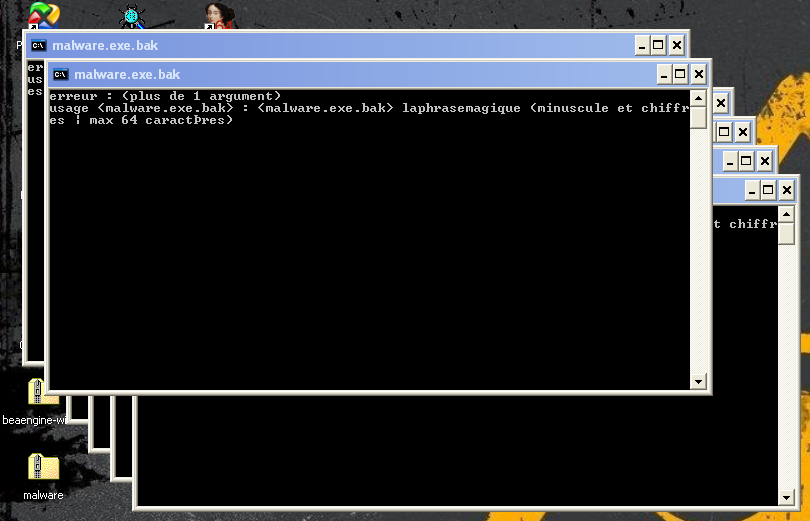
\includegraphics[width=\textwidth]{fork-bomb.png}
\end{figure}

Si le programme détecte qu'il est débuggé, il fait une suite d'actions:
- Ouvre un fichier "aa.txt" avec notepad (chaîne trouvée plus tôt)
- Bloque les entrées du clavier et de la souris (on ne peut plus interagir avec l'ordinateur) pour les applications
- Bloque les entées du clavier et de la souris pour la fenêtre courante
- Quitte

\subsection{Deboggage}
A chaque test anti-debug rencontré, on a inversé la condition.
On a executé pas-à-pas le programme pour voir comment était traitée notre chaîne d'entrée.
On a trouvé une fonction qui "hash" l'entrée (cf. plus haut)
Puis une fonction qui compare le haché avec le haché de la clé.

\subsection{Bruteforce}

Il nous a donc suffit de réimplémenter l'algorithme de hachage et de bruteforcer différentes combinaisons de clé pour trouver des combinaisons valides.
Premier match en 30 minutes: "tmmm3ri", 400 matchs en deux jours, et 1000 en 5/6 jours.

\end{document} 